\documentclass[11pt,a4paper]{article}

\usepackage{graphicx}
\usepackage{url}
\usepackage{listings}
\title{Interface DC motor using motor driver IC to the Raspberry Pi }
\author{e-Yantra Team}
\date{\today}


\begin{document}
	\maketitle
	\newpage
	\tableofcontents
	\newpage
	\section{Objective}
	In this tutorial we shall learn to control the velocity of DC motors interfaced with Raspberry Pi using a motor driver IC.
	
	\section{Prerequisites}
	\begin{itemize}
		\item Python programming skills
		\item An R-Pi (with I2C; I will be using version 2 ) 
		\item An idea about working of a dc motor
		\item Interfacing an MCP23017 IC with an R-Pi should be known
	\end{itemize}
	
	\section{Hardware Requirement}
	\begin{enumerate}
		\item Raspberry Pi (I will be using Version 2 Model B+)
		\item MCP23017
		\item Power adapter
	    \item DC motor
	    \item L293D
	    \item Capacitors (0.1 uF)
	    \item External power supply (for 12V)
	    \item Connecting wires
		\item Bread board
	\end{enumerate}
	
	\section{Software Requirement}
	\begin{enumerate}
		\item PyScripter (version 2.7 or above)
		\item Mobaxterm (for windows user)
	\end{enumerate}
	
	\newpage
	\section{Theory and Description}
	A DC motor is any of a class of electrical machines that converts direct current electrical power into mechanical power. The most common types rely on the forces produced by magnetic fields. Nearly all types of DC motors have some internal mechanism, either electromechanical or electronic, to periodically change the direction of current flow in part of the motor. Most types produce rotary motion; a linear motor directly produces force and motion in a straight line.
	
	\vspace{0.5cm}
	\flushleft
	\textbf{Motor Driver}
	\vspace{0.3cm}
	\newline
	Normal DC gear-head motors require current greater than 250mA. Most of the ICs like 555 timer,74 series ICs cannot supply this amount of current.Instead if we directly connect motors to the output of any of the above IC's, they might get damaged. There is a need of a circuitry that can act as a bridge between the above mentioned ICs and the motors. This is where a motor driver plays a crucial role. It regulates the current flowing through the circuit hence preventing any damage to the device.
	
	Different motor driver circuits can be classified as ones:
	\begin{itemize}
		\item Using Transistor
		\item Using L293D/L298
		\item Using relays
	\end{itemize}
    
    \newpage
    For controlling motor in both directions H bridge circuit is used. Its working is very simple and is described below.
    \begin{figure}[h!]
    	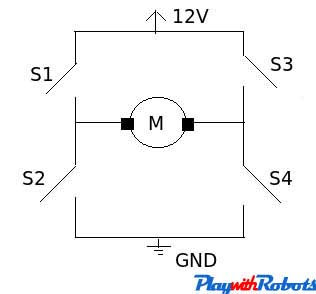
\includegraphics[scale=1]{hb.jpg}
    	\centering
    	\caption{[2]}
    \end{figure} 
    
    \begin{tabular}{|c|c|c|c|}
    	\hline
	    Closed Switches & Open Switches & Voltage across motor & Motion\\
	    \hline
		Nil	& S1,S2,S3,S4	& 0 & No motion\\
		\hline
	    S1,S4 &	S2,S3 &	12V & Clockwise \\
	    \hline
	    S2,S3 & S1,S4 & -12V & Anti-clockwise \\
	    \hline
	    S1,S3 & S2,S4 & 0V & Brake\\
	    \hline
    \end{tabular}
    \centering
    Ref: [2]
    
    \newpage
    \flushleft
    \textbf{L293D Motor Driver}
    \vspace{0.3cm}
    \newline
    L293D is dual H-bridge motor driver ICs. Using these we can control the rotation of two motors in both clockwise and anti-clockwise direction.
    
    \vspace{0.3cm}
    \textbf{Pin configuration}
    \begin{figure}[h!]
    	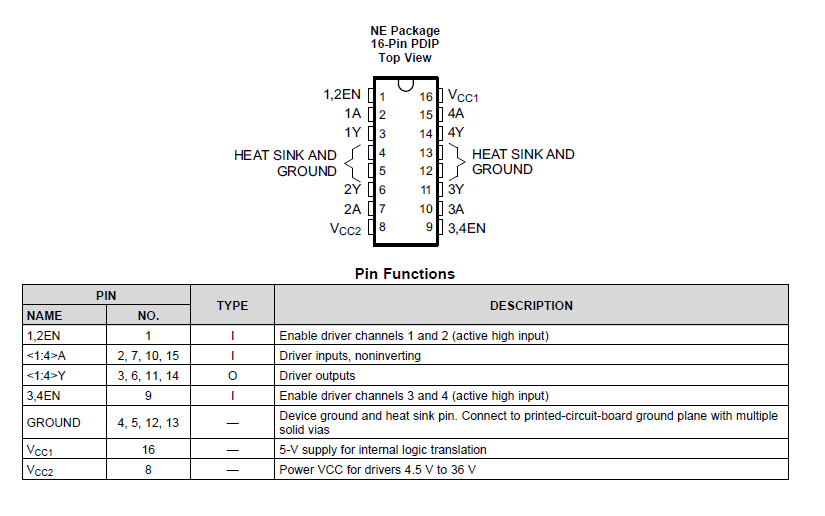
\includegraphics[scale=0.7]{l293d_with_pinfun.png}
    	\centering
    	\caption{[2]}
    \end{figure}
    
    The description of each pin is as follows:
    \begin{itemize}
    	\item Enable pins: These are pin no. 1 and pin no. 9. Pin no. 1 is used to enable Half-H driver 1 and 2.( H bridge on Left side). Pin no. 9 is used to enable H-bridge driver 3and 4.(H bridge on right side). The concept is simple, if you want to use a particular H bridge you have to give a high logic to corresponding enable pins along with the power supply to the IC. This pin can also be used to control speed of the motor using PWM technique.
    	\item VCC1 (Pin 16): Power supply pin. Connect it to 5V supply.
    	\item VCC2 (Pin 8): Power supply for motor. Apply +ve voltage to it as per motor rating. If you want to drive your motor at 12V, apply 12V on this pin. It is also possible to drive motor directly on a battery, other than the one used for supplying power to the circuit, Just connect +ve terminal of that battery to VCC2 pin and make GND of both the batteries common. (MAX voltage at this pin is 36V as per its datasheet).
    	\item GND (Pins 4,5,12,13): Connect them to common GND of circuit.
    	\item Inputs (Pins 2,7,10,15): These are input pins through which control signals are given by microcontrollers or other circuits/ICs. For example, if on pin 2 (Input of 1st half H driver) we give Logic 1 ( 5V), we will get a voltage equal to VCC2 on corresponding output pin of 1st half H driver i.e pin no. 3. Similarly for Logic 0 (0V) on Pin 2, 0V on Pin 3 appears.
    	\item Outputs ( Pin 3,6,11,14): Outputs pins. According to input signal output signal comes. [2]
    \end{itemize}
    
    \vspace{0.3cm}
    \textbf{Circuit Diagram}
    
    \begin{figure}[h!]
    	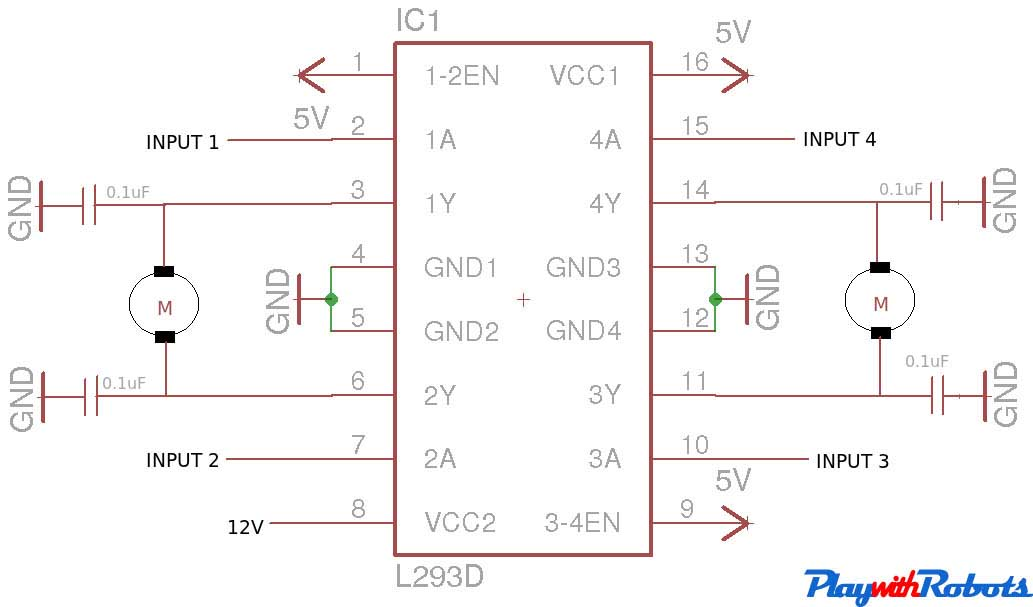
\includegraphics[scale=0.5]{lc.jpg}
    	\centering
    	\caption{[2]}
    \end{figure}
    
    \vspace{0.5cm}
    \centering
    \begin{tabular}{|c|c|c|c|c|}
    	\hline
    	1A & 2A	& 1Y & 2Y & Motor 1\\
    	\hline
    	Logic 0	& Logic 0 & 0 & 0 & Stop \\
    	\hline
    	Logic 1	& Logic 0 & 12V	& 0	& Clockwise\\
    	\hline
    	Logic 0	& Logic 1 & 0 & 12V	& Anti-clockwise\\
    	\hline
    	Logic 1	& Logic 1 & 12V & 12V & Brake\\
    	\hline
    \end{tabular}
    \newline
    Ref: [2]
    
    \newpage
    \flushleft 
	\section{Experiment}
		\subsection{ DC motor interfaced with Raspberry Pi through L293D and MCP23017 IC}
	In this experiment we will be rotating the DC motor in both direction by using MCP23017(Port Expander IC) and L293D(Motor Driver IC).
	  
	\begin{figure}[h!]
		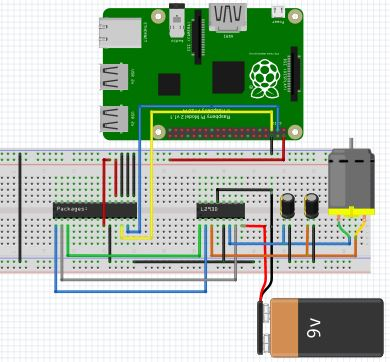
\includegraphics[scale=0.6]{DC_motor_I2C.jpg}
		\centering
	\end{figure} 
	As shown in the figure:
	\begin{itemize}
		\item Pin 9 (VDD) is connected to 5V (Red)
		\item Pin 10 (VSS) is connected to Ground (Black)
		\item Pin 12 (SCL) is connected to Pin 5 on the Pi GPIO (Blue)
		\item Pin 13 (SDA) is connected to Pin 3 on the Pi GPIO (Blue)
		\item Pin 18 (Reset) should be set high for normal operation so we connect this to 5V (Red)
		\item Pins 15, 16 \& 17 (A0-A2) determine the number assigned to this device. We are only using one device so we will give it a binary zero by setting all three of these pins to 0 (ground) (Black)
		\item Input 1 and Input 2 of L293D is connected to GPB0 and GPB1 of MCP23017 (Orange)
		\item Pin 1 (enable pin) of L293D is connected to GPB2.
		\item Out 1 and Out 2 are connected to a DC motor
	\end{itemize}
	
	\newpage 
	\textbf{Code}
	\vspace{0.3cm}
	
	\lstinputlisting[language=Python]{DC_motor_I2C_test.py}
	
	\newpage
	\section{Appendix}
	
	\subsection{Raspberry Pi 2 Pin-out Diagram}
	\begin{figure}[h!]
		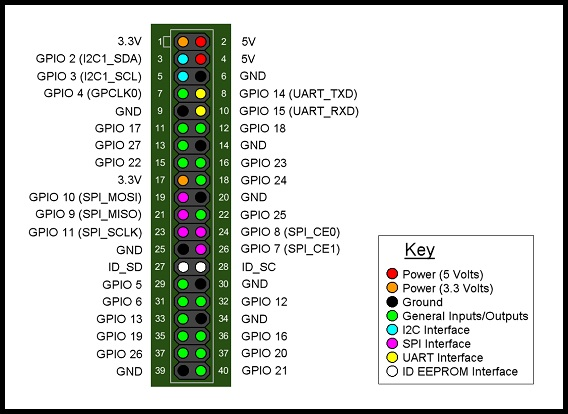
\includegraphics[scale=0.6]{RaspberryPi2_pinout.jpg}
		\centering
		\caption{[4]}
	\end{figure}
	\subsection{L293D Pinouts}
	\begin{figure}[h!]
		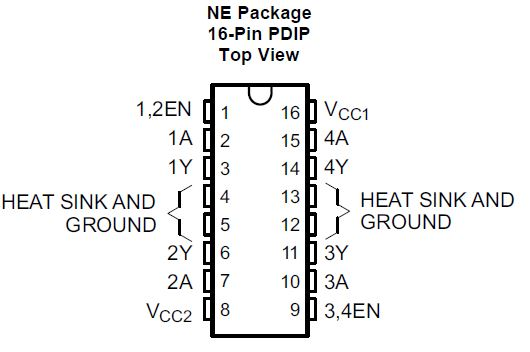
\includegraphics[scale=0.6]{l293d.jpg}
		\centering
		\caption{[4]}
	\end{figure}
	
	\subsection{MCP23017 datasheet}
	
	\url{http://ww1.microchip.com/downloads/en/DeviceDoc/21952b.pdf}
	\subsection{L293D datasheet}
	
	\url{http://www.ti.com/lit/ds/symlink/l293.pdf}
	\subsection{MCP23017}
	\url{http://ww1.microchip.com/downloads/en/DeviceDoc/21952b.pdf}
	
	\section{References}
	\begin{enumerate}
		\item \url{https://en.wikipedia.org/wiki/DC_motor}
		\item \url{http://playwithrobots.com/dc-motor-driver-circuits/}
		\item \url{http://www.electronics-tutorials.ws/blog/pulse-width-modulation.html}
		\item \url{http://data.designspark.info/uploads/images/53bc258dc6c0425cb44870b50ab30621}
	\end{enumerate}
	
\end{document}



